%%%%%%%%%%%%%%%%%%%%%%%%%%%%%%%%%%%%%%%%%
% University Assignment Title Page 
% LaTeX Template
% Version 1.0 (27/12/12)
%
% This template has been downloaded from:
% http://www.LaTeXTemplates.com
%
% Original author:
% WikiBooks (http://en.wikibooks.org/wiki/LaTeX/Title_Creation)
%
% License:
% CC BY-NC-SA 3.0 (http://creativecommons.org/licenses/by-nc-sa/3.0/)
% 
% Instructions for using this template:
% This title page is capable of being compiled as is. This is not useful for 
% including it in another document. To do this, you have two options: 
%
% 1) Copy/paste everything between \begin{document} and \end{document} 
% starting at \begin{titlepage} and paste this into another LaTeX file where you 
% want your title page.
% OR
% 2) Remove everything outside the \begin{titlepage} and \end{titlepage} and 
% move this file to the same directory as the LaTeX file you wish to add it to. 
% Then add %%%%%%%%%%%%%%%%%%%%%%%%%%%%%%%%%%%%%%%%%
% University Assignment Title Page 
% LaTeX Template
% Version 1.0 (27/12/12)
%
% This template has been downloaded from:
% http://www.LaTeXTemplates.com
%
% Original author:
% WikiBooks (http://en.wikibooks.org/wiki/LaTeX/Title_Creation)
%
% License:
% CC BY-NC-SA 3.0 (http://creativecommons.org/licenses/by-nc-sa/3.0/)
% 
% Instructions for using this template:
% This title page is capable of being compiled as is. This is not useful for 
% including it in another document. To do this, you have two options: 
%
% 1) Copy/paste everything between \begin{document} and \end{document} 
% starting at \begin{titlepage} and paste this into another LaTeX file where you 
% want your title page.
% OR
% 2) Remove everything outside the \begin{titlepage} and \end{titlepage} and 
% move this file to the same directory as the LaTeX file you wish to add it to. 
% Then add %%%%%%%%%%%%%%%%%%%%%%%%%%%%%%%%%%%%%%%%%
% University Assignment Title Page 
% LaTeX Template
% Version 1.0 (27/12/12)
%
% This template has been downloaded from:
% http://www.LaTeXTemplates.com
%
% Original author:
% WikiBooks (http://en.wikibooks.org/wiki/LaTeX/Title_Creation)
%
% License:
% CC BY-NC-SA 3.0 (http://creativecommons.org/licenses/by-nc-sa/3.0/)
% 
% Instructions for using this template:
% This title page is capable of being compiled as is. This is not useful for 
% including it in another document. To do this, you have two options: 
%
% 1) Copy/paste everything between \begin{document} and \end{document} 
% starting at \begin{titlepage} and paste this into another LaTeX file where you 
% want your title page.
% OR
% 2) Remove everything outside the \begin{titlepage} and \end{titlepage} and 
% move this file to the same directory as the LaTeX file you wish to add it to. 
% Then add %%%%%%%%%%%%%%%%%%%%%%%%%%%%%%%%%%%%%%%%%
% University Assignment Title Page 
% LaTeX Template
% Version 1.0 (27/12/12)
%
% This template has been downloaded from:
% http://www.LaTeXTemplates.com
%
% Original author:
% WikiBooks (http://en.wikibooks.org/wiki/LaTeX/Title_Creation)
%
% License:
% CC BY-NC-SA 3.0 (http://creativecommons.org/licenses/by-nc-sa/3.0/)
% 
% Instructions for using this template:
% This title page is capable of being compiled as is. This is not useful for 
% including it in another document. To do this, you have two options: 
%
% 1) Copy/paste everything between \begin{document} and \end{document} 
% starting at \begin{titlepage} and paste this into another LaTeX file where you 
% want your title page.
% OR
% 2) Remove everything outside the \begin{titlepage} and \end{titlepage} and 
% move this file to the same directory as the LaTeX file you wish to add it to. 
% Then add \input{./title_page_1.tex} to your LaTeX file where you want your
% title page.
%
%%%%%%%%%%%%%%%%%%%%%%%%%%%%%%%%%%%%%%%%%
%\title{Title page with logo}
%----------------------------------------------------------------------------------------
%	PACKAGES AND OTHER DOCUMENT CONFIGURATIONS
%----------------------------------------------------------------------------------------

\documentclass[12pt]{article}
\usepackage[english]{babel}
\usepackage[utf8x]{inputenc}
\usepackage{amsmath}
\usepackage{graphicx}
\usepackage[colorinlistoftodos]{todonotes}
\usepackage{listings}
\usepackage{hyperref}

\hypersetup{
    colorlinks=true,
    linkcolor=blue,
    filecolor=magenta,      
    urlcolor=cyan,
}

\lstset{
  backgroundcolor = \color{lightgray},
  basicstyle=\ttfamily,
  columns=fullflexible,
  breaklines=true,
  postbreak=\mbox{\textcolor{red}{$\hookrightarrow$}\space},
}


\begin{document}

\begin{titlepage}

\newcommand{\HRule}{\rule{\linewidth}{0.5mm}} % Defines a new command for the horizontal lines, change thickness here

\center % Center everything on the page
 
%----------------------------------------------------------------------------------------
%	HEADING SECTIONS
%----------------------------------------------------------------------------------------

\textsc{\LARGE Politenico di Milano}\\[1.5cm] % Name of your university/college
\textsc{\Large Dipartimento Elettronica, Informazione e Bioingegneria}\\[0.5cm] % Major heading such as course name
\textsc{\large HEAPLab Project Report}\\[0.5cm] % Minor heading such as course title

%----------------------------------------------------------------------------------------
%	TITLE SECTION
%----------------------------------------------------------------------------------------

\HRule \\[0.4cm]
{ \huge \bfseries Needleman-Wunsch\\algorithm sample\\for Mango OpenCL}\\[0.4cm] % Title of your document
\HRule \\[1.5cm]
 
%----------------------------------------------------------------------------------------
%	AUTHOR SECTION
%----------------------------------------------------------------------------------------

\begin{minipage}{0.4\textwidth}
\begin{flushleft} \large
\emph{Author:}\\
Luca \textsc{Gambarotto} % Your name
\end{flushleft}
\end{minipage}
~
\begin{minipage}{0.4\textwidth}
\begin{flushright} \large
\emph{Supervisor:} \\
Dr. Giuseppe \textsc{Massari} % Supervisor's Name
\end{flushright}
\end{minipage}\\[2cm]

% If you don't want a supervisor, uncomment the two lines below and remove the section above
%\Large \emph{Author:}\\
%John \textsc{Smith}\\[3cm] % Your name

%----------------------------------------------------------------------------------------
%	DATE SECTION
%----------------------------------------------------------------------------------------

{\large \today}\\[1.3cm] % Date, change the \today to a set date if you want to be precise

%----------------------------------------------------------------------------------------
%	LOGO SECTION
%----------------------------------------------------------------------------------------


\includegraphics[width=100pt]{heaplogo.pdf}\\[1cm] % Include a department/university logo - this will require the graphicx package
 
%----------------------------------------------------------------------------------------

\vfill % Fill the rest of the page with whitespace

\end{titlepage}




\begin{abstract}
This project is aimed at coding and building a complete sample application using the OpenCL implementation offered by Mango. Specifically the application developed is a porting of the OpenCL implementation of the Needleman-Wunsch algorithm proposed in the Rodinia Benchmark Suite\cite{rodinia}.\\The development of the project, aside from the pure code drawing up, allowed me to dig into the technologies for parallel coding, both hardware and software side, dealing with topics that are not usually covered in mandatory courses at Politecnico di Milano.


\end{abstract}

\section{Introduction}

\subsection{The objective}
The main objective of the present project is to provide a complete and clear implementation of an application developed using the OpenCL libraries provided by Mango. The main idea that guided the development was to produce a sort of "scaffolding" that will allow developers to easily develop different applications using the same libraries.

\subsection{The Needleman-Wunsch algorithm}
The Needleman-Wunsch algorithm is used to compare two sequences of symbols and find out how much similar they are, using a specific metric and similarity values. It is particularly useful in bioinformatics, to compare and align sequences of proteins or nucleotides. It is largely used in the development of vaccines and in the monitoring of the evolution of viruses.\\The original version proposed was not meant to be parallelized. During the years, seen the benefit of its use, some improvements have been proposed. The original sample, developed both for OpenCL and Cuda and included in the Rodinia Benchmark Suite, is a limited and simplified version that allows to exploit multi-processor computation.\\For futher details about the NW algorithm see the document\cite{nw} in the reference section.

\section{Design and Implementation}

The sample has been design to provide the same functionalities of the original one, to allow the developers to easily compare the code of a "plain" OpenCL application to the one of an application developed using Mango. In particular these aspects has been kept unchanged:
\begin{itemize}
      \item The input sequences can be only randomly generated and their length must be a multiple of 16. Altough the new sample is therically able to manage sequences of arbitrary length, the limitation of the original application has been kept.
      \item The substitution matrix, used by the algorithm to give an evalutation of similarity between two elements of the sequences, has been kept unchanged. In particular it is the blosum62 matrix, a popular substitution matrix often used with these kinds of algorithm. Even if it is a 24 by 24 matrix, meaning that can potentially compare elements from a library of 24 symbols, only the upper-left 11 by 11 part of the matrix is actually used by the sample, as in the original application.
      \item As for the original application, the penalty value to be used must be specified in the arguments passed to executable.
\end{itemize}
Despite the behavior and the functionalities are the same, the application has been enriched with the possibility of visualizing the results obtained through the automatic generation of a .txt file containing the trackeback matrix computed and the actual traceback sequence.

Far what the device part is concerned, the original code was divided in two kernels, one working on the upper-left part of the trace-back matrix and one working on the lower-right one. Exploiting the possibilities offered by Mango, these two kernels have been unified in a single function, pre-compiled during the setup of the samples and stored in the mango installation directory.

With respect to the original application, the code has been completely re-arranged, splitting the setup parts of the code in several function whose goals is to provide a starting point for future Mango applications.


\section{Troubleshooting}
During the setup of the enviroment (BarbequeRTRM and Mango) on my machine, following the instructions in the documentation, I've encountered some small issues. Here is a list of the most notable ones, with the solution I've found to solve them.

\subsection{Kconfig error}
During the setup of the Mango/BarbequeRTRM enviroment the procedure got stuck with the following errors:
\begin{lstlisting}[language=bash]
      $ build/platforms/Kconfig:120:warning: environment variable OCLROOT undefined//
      $ build/platforms/Kconfig:137:warning: environment variable NVML_ROOT_DIR undefined//
      $ build/configuration/Kconfig-external:3: can't open file "build/configuration/Kconfig-external-required"
\end{lstlisting}

To solve the first two I simly manually added the required environment variables, setting them to an empty value, using the following terminal commands:

\begin{lstlisting}[language=bash]
      $ export OCLROOT=
\end{lstlisting}

\begin{lstlisting}[language=bash]
      $ export NVML_ROOT_DIR=
\end{lstlisting}

For what the last error is concerned, I noticed that it appears only using ubuntu 19.10 while on the version 18.04 LTS (the last LTS version at the time I set my system up) it does not arise. This is probably due to the fact that some libraries required by the setup has been changed. To confirm that the problem was actually the distribution I was installing the framework on I tried both versions in a virtual machine, replicating the same commands in parallel on thetwo systems.

\subsection{Library path environment variable missing}
The execution of a compiled opencl sample returns the following error (in this case the executable run is the Needleman-Wunsch sample but the problem also happens with any other sample).

\begin{lstlisting}[language=bash]
      $ ./nw_opencl: symbol lookup error: ./nw_opencl: undefined symbol: clStartComputation
\end{lstlisting}

To solve the issue it is enough to manually add the LD\_LIBRARY\_PATH environment variable in the system and populate it with the path where the mangolibs are installed, using the following command:

\begin{lstlisting}[language=bash]
      $ export LD_LIBRARY_PATH = /opt/mango/usr/local/lib
\end{lstlisting}

\section{Experimental Results}

The development of this sample and the finished sample itself can be analyzed in several ways: in addition to the considerations on the raw performances, in terms of "speed" and flexibility compared to the original OpenCL version, some interesting spotlights can be placed also on the complexity of the code, in terms of effort needed to become familiar with the libraries, and on the framework itself.

\subsection{Performances}
For what the performaces of the new code compared to the original OpenCL version are concerned, considerations can be carried on (or, at least, a comparison can be supposed) on two different areas:
\begin{itemize}
      \item Pure speed (in terms of milliseconds needed to complete the task): since the original OpenCL implementation is quite limited (only short sequences can be compared) no valuable estimation of the execution time can be measured.
      \item Flexibility of the code: while the original sample, without modifications, was only able to run comparison of sequences of at most 256 charecters before run out of resources on my thesting machine (equipped with an old but still efficient Intel Sandy Bridge processor) the ported sample is able to run also with longer sequences (here, as a proof, is attached the log for a sequence of 1024 characters, but I was able to complete the execution also on longer sequences). This means that, on a comparable code complexity, the Mango framework (OpenCL implementation and backend BarbequeRTRM) is able to solve problems that are quantitatively more complex (i.e. problems related with bigger matrices).
\end{itemize}


\subsection{Code complexity}
Considering the outcome of the project not only the finished code but also the process that lead it, we can also analyze the learning curve and the difficulties that a developer interested in the mango framework can encounter:
\begin{itemize}
      \item Looking at the host-side code the library, a developer with basic knowledge on OpenCL can easily adapt to the differences of the mango libraries.
      \item Moving to the kernel (the device-side code) the code is way more easy: while in plain OpenCL it is necessary to manually decompose the problem and think to a code that can be parallelized, in mango it is enough to write a C-like function containing a loop. This allows the developer to easily implement their code, abstracting from all the underlying complexity due to the parallelization.
\end{itemize}


\section{Conclusions}
\subsection{Addititional topics covered}
Beside the development of the raw code, this project allowed me to learn (or, at least, to get a glance and study) the following topics:
\begin{itemize}
      \item High-performance hardware: since the original topic for the project, changed due to the pandemic, was related to a high-performance computing board with an integrated hardware accelerator (the Parallelaboard), I spent some weeks digging in the documentation provided by Adapteva.
      Even if this provided to be superfluous in the end, allowed me to grasp some concepts that turned out to be useful anyway. E.g. the way the data exchange between the host processor and the accelerator turned out to be very similar to what is the behavior of OpenCL. Furthermore the concept of using two different pieces of the code, one for the orchestrator (the host) and one for the device (the accelerator) allowed me to better understand what kernels are in OpenCL.
      \item OpenCL: to fully understand the original code of the sample I took to opportunity to deepen this topic. Even if Mango libraries are quite different w.r.t. the plain OpenCL, especially for what the kernels are concerned, I made several trials on OpenCL too, to add basic concepts of this framework in my background\cite{oclmanual}.
      \item Kconfig and CMake: despite being marginal in the development of the core project I had the opportunity of taking a grasp of these two tools.
\end{itemize}


\section{The Parallelaboard}
Before the Covid pandemic outbreak, and the consequent change in the topic of the project due to the impossibility of reaching the Politecnico campus, I started to study the possibility of porting the BarbequeRTRM framework to the Adapteva Epiphany III Parallelaboard, an ambedded development board with a many-core accelerator. To understand the architecture of the board I found useful an old thesis\cite{pb2} where the board possibilities are well described, both in terms of hardware and software.\\In particular I have considered two opportunities:
\begin{itemize}
      \item Exploit the functions provided by the SDK libraries\cite{pb1} to implement a platform proxy for BarbequeRTRM. Unfortunately this approach doesn't seem to be promising since the possibilities of controlling the boards are quite limited (there are no functions to retrieve the temperatures, the power consumption or the control of fan eventually installed on the board).
      \item Exploit the OpenCL libraries developed for the Epiphany accelerator\cite{pb3}: although the development was stopped in 2013, there exists an unofficial implementation of the openCL libraries that may be useful to allow the board to be used with mango OpenCL applications (such as the one I developed).
\end{itemize}

\begin{thebibliography}{9}

      \bibitem{rodinia}
            \textit{Rodinia Benchmark Suite},
            \url{https://rodinia.cs.virginia.edu/doku.php}
      
      \bibitem{oclmanual}
            \textit{Khronos openCL reference guide},
            \url{https://man.opencl.org}
      
      \bibitem{nw}
            Vladimir Likic - 
            \textit{The Needleman-Wunsch algo. for sequence alignment},
            \url{https://www.cs.sjsu.edu/~aid/cs152/NeedlemanWunsch.pdf}


      \bibitem{pb1}
            \textit{ParallelaBoard SDK manual},
            \url{https://adapteva.com/docs/epiphany_sdk_ref.pdf}
            
      \bibitem{pb2}
            Adriano Cardace -
            \textit{Implementazione del modello di Biham-Middleton-Levine sulla Parallella Board},
            \url{https://amslaurea.unibo.it/14383/1/Adriano-Cardace-tesi.pdf}

      \bibitem{pb3}
            \textit{ParallelaBoard - OpenCL framework implementation},
            \url{https://github.com/browndeer/coprthr}

            

\end{thebibliography}

\end{document} to your LaTeX file where you want your
% title page.
%
%%%%%%%%%%%%%%%%%%%%%%%%%%%%%%%%%%%%%%%%%
%\title{Title page with logo}
%----------------------------------------------------------------------------------------
%	PACKAGES AND OTHER DOCUMENT CONFIGURATIONS
%----------------------------------------------------------------------------------------

\documentclass[12pt]{article}
\usepackage[english]{babel}
\usepackage[utf8x]{inputenc}
\usepackage{amsmath}
\usepackage{graphicx}
\usepackage[colorinlistoftodos]{todonotes}
\usepackage{listings}
\usepackage{hyperref}

\hypersetup{
    colorlinks=true,
    linkcolor=blue,
    filecolor=magenta,      
    urlcolor=cyan,
}

\lstset{
  backgroundcolor = \color{lightgray},
  basicstyle=\ttfamily,
  columns=fullflexible,
  breaklines=true,
  postbreak=\mbox{\textcolor{red}{$\hookrightarrow$}\space},
}


\begin{document}

\begin{titlepage}

\newcommand{\HRule}{\rule{\linewidth}{0.5mm}} % Defines a new command for the horizontal lines, change thickness here

\center % Center everything on the page
 
%----------------------------------------------------------------------------------------
%	HEADING SECTIONS
%----------------------------------------------------------------------------------------

\textsc{\LARGE Politenico di Milano}\\[1.5cm] % Name of your university/college
\textsc{\Large Dipartimento Elettronica, Informazione e Bioingegneria}\\[0.5cm] % Major heading such as course name
\textsc{\large HEAPLab Project Report}\\[0.5cm] % Minor heading such as course title

%----------------------------------------------------------------------------------------
%	TITLE SECTION
%----------------------------------------------------------------------------------------

\HRule \\[0.4cm]
{ \huge \bfseries Needleman-Wunsch\\algorithm sample\\for Mango OpenCL}\\[0.4cm] % Title of your document
\HRule \\[1.5cm]
 
%----------------------------------------------------------------------------------------
%	AUTHOR SECTION
%----------------------------------------------------------------------------------------

\begin{minipage}{0.4\textwidth}
\begin{flushleft} \large
\emph{Author:}\\
Luca \textsc{Gambarotto} % Your name
\end{flushleft}
\end{minipage}
~
\begin{minipage}{0.4\textwidth}
\begin{flushright} \large
\emph{Supervisor:} \\
Dr. Giuseppe \textsc{Massari} % Supervisor's Name
\end{flushright}
\end{minipage}\\[2cm]

% If you don't want a supervisor, uncomment the two lines below and remove the section above
%\Large \emph{Author:}\\
%John \textsc{Smith}\\[3cm] % Your name

%----------------------------------------------------------------------------------------
%	DATE SECTION
%----------------------------------------------------------------------------------------

{\large \today}\\[1.3cm] % Date, change the \today to a set date if you want to be precise

%----------------------------------------------------------------------------------------
%	LOGO SECTION
%----------------------------------------------------------------------------------------


\includegraphics[width=100pt]{heaplogo.pdf}\\[1cm] % Include a department/university logo - this will require the graphicx package
 
%----------------------------------------------------------------------------------------

\vfill % Fill the rest of the page with whitespace

\end{titlepage}




\begin{abstract}
This project is aimed at coding and building a complete sample application using the OpenCL implementation offered by Mango. Specifically the application developed is a porting of the OpenCL implementation of the Needleman-Wunsch algorithm proposed in the Rodinia Benchmark Suite\cite{rodinia}.\\The development of the project, aside from the pure code drawing up, allowed me to dig into the technologies for parallel coding, both hardware and software side, dealing with topics that are not usually covered in mandatory courses at Politecnico di Milano.


\end{abstract}

\section{Introduction}

\subsection{The objective}
The main objective of the present project is to provide a complete and clear implementation of an application developed using the OpenCL libraries provided by Mango. The main idea that guided the development was to produce a sort of "scaffolding" that will allow developers to easily develop different applications using the same libraries.

\subsection{The Needleman-Wunsch algorithm}
The Needleman-Wunsch algorithm is used to compare two sequences of symbols and find out how much similar they are, using a specific metric and similarity values. It is particularly useful in bioinformatics, to compare and align sequences of proteins or nucleotides. It is largely used in the development of vaccines and in the monitoring of the evolution of viruses.\\The original version proposed was not meant to be parallelized. During the years, seen the benefit of its use, some improvements have been proposed. The original sample, developed both for OpenCL and Cuda and included in the Rodinia Benchmark Suite, is a limited and simplified version that allows to exploit multi-processor computation.\\For futher details about the NW algorithm see the document\cite{nw} in the reference section.

\section{Design and Implementation}

The sample has been design to provide the same functionalities of the original one, to allow the developers to easily compare the code of a "plain" OpenCL application to the one of an application developed using Mango. In particular these aspects has been kept unchanged:
\begin{itemize}
      \item The input sequences can be only randomly generated and their length must be a multiple of 16. Altough the new sample is therically able to manage sequences of arbitrary length, the limitation of the original application has been kept.
      \item The substitution matrix, used by the algorithm to give an evalutation of similarity between two elements of the sequences, has been kept unchanged. In particular it is the blosum62 matrix, a popular substitution matrix often used with these kinds of algorithm. Even if it is a 24 by 24 matrix, meaning that can potentially compare elements from a library of 24 symbols, only the upper-left 11 by 11 part of the matrix is actually used by the sample, as in the original application.
      \item As for the original application, the penalty value to be used must be specified in the arguments passed to executable.
\end{itemize}
Despite the behavior and the functionalities are the same, the application has been enriched with the possibility of visualizing the results obtained through the automatic generation of a .txt file containing the trackeback matrix computed and the actual traceback sequence.

Far what the device part is concerned, the original code was divided in two kernels, one working on the upper-left part of the trace-back matrix and one working on the lower-right one. Exploiting the possibilities offered by Mango, these two kernels have been unified in a single function, pre-compiled during the setup of the samples and stored in the mango installation directory.

With respect to the original application, the code has been completely re-arranged, splitting the setup parts of the code in several function whose goals is to provide a starting point for future Mango applications.


\section{Troubleshooting}
During the setup of the enviroment (BarbequeRTRM and Mango) on my machine, following the instructions in the documentation, I've encountered some small issues. Here is a list of the most notable ones, with the solution I've found to solve them.

\subsection{Kconfig error}
During the setup of the Mango/BarbequeRTRM enviroment the procedure got stuck with the following errors:
\begin{lstlisting}[language=bash]
      $ build/platforms/Kconfig:120:warning: environment variable OCLROOT undefined//
      $ build/platforms/Kconfig:137:warning: environment variable NVML_ROOT_DIR undefined//
      $ build/configuration/Kconfig-external:3: can't open file "build/configuration/Kconfig-external-required"
\end{lstlisting}

To solve the first two I simly manually added the required environment variables, setting them to an empty value, using the following terminal commands:

\begin{lstlisting}[language=bash]
      $ export OCLROOT=
\end{lstlisting}

\begin{lstlisting}[language=bash]
      $ export NVML_ROOT_DIR=
\end{lstlisting}

For what the last error is concerned, I noticed that it appears only using ubuntu 19.10 while on the version 18.04 LTS (the last LTS version at the time I set my system up) it does not arise. This is probably due to the fact that some libraries required by the setup has been changed. To confirm that the problem was actually the distribution I was installing the framework on I tried both versions in a virtual machine, replicating the same commands in parallel on thetwo systems.

\subsection{Library path environment variable missing}
The execution of a compiled opencl sample returns the following error (in this case the executable run is the Needleman-Wunsch sample but the problem also happens with any other sample).

\begin{lstlisting}[language=bash]
      $ ./nw_opencl: symbol lookup error: ./nw_opencl: undefined symbol: clStartComputation
\end{lstlisting}

To solve the issue it is enough to manually add the LD\_LIBRARY\_PATH environment variable in the system and populate it with the path where the mangolibs are installed, using the following command:

\begin{lstlisting}[language=bash]
      $ export LD_LIBRARY_PATH = /opt/mango/usr/local/lib
\end{lstlisting}

\section{Experimental Results}

The development of this sample and the finished sample itself can be analyzed in several ways: in addition to the considerations on the raw performances, in terms of "speed" and flexibility compared to the original OpenCL version, some interesting spotlights can be placed also on the complexity of the code, in terms of effort needed to become familiar with the libraries, and on the framework itself.

\subsection{Performances}
For what the performaces of the new code compared to the original OpenCL version are concerned, considerations can be carried on (or, at least, a comparison can be supposed) on two different areas:
\begin{itemize}
      \item Pure speed (in terms of milliseconds needed to complete the task): since the original OpenCL implementation is quite limited (only short sequences can be compared) no valuable estimation of the execution time can be measured.
      \item Flexibility of the code: while the original sample, without modifications, was only able to run comparison of sequences of at most 256 charecters before run out of resources on my thesting machine (equipped with an old but still efficient Intel Sandy Bridge processor) the ported sample is able to run also with longer sequences (here, as a proof, is attached the log for a sequence of 1024 characters, but I was able to complete the execution also on longer sequences). This means that, on a comparable code complexity, the Mango framework (OpenCL implementation and backend BarbequeRTRM) is able to solve problems that are quantitatively more complex (i.e. problems related with bigger matrices).
\end{itemize}


\subsection{Code complexity}
Considering the outcome of the project not only the finished code but also the process that lead it, we can also analyze the learning curve and the difficulties that a developer interested in the mango framework can encounter:
\begin{itemize}
      \item Looking at the host-side code the library, a developer with basic knowledge on OpenCL can easily adapt to the differences of the mango libraries.
      \item Moving to the kernel (the device-side code) the code is way more easy: while in plain OpenCL it is necessary to manually decompose the problem and think to a code that can be parallelized, in mango it is enough to write a C-like function containing a loop. This allows the developer to easily implement their code, abstracting from all the underlying complexity due to the parallelization.
\end{itemize}


\section{Conclusions}
\subsection{Addititional topics covered}
Beside the development of the raw code, this project allowed me to learn (or, at least, to get a glance and study) the following topics:
\begin{itemize}
      \item High-performance hardware: since the original topic for the project, changed due to the pandemic, was related to a high-performance computing board with an integrated hardware accelerator (the Parallelaboard), I spent some weeks digging in the documentation provided by Adapteva.
      Even if this provided to be superfluous in the end, allowed me to grasp some concepts that turned out to be useful anyway. E.g. the way the data exchange between the host processor and the accelerator turned out to be very similar to what is the behavior of OpenCL. Furthermore the concept of using two different pieces of the code, one for the orchestrator (the host) and one for the device (the accelerator) allowed me to better understand what kernels are in OpenCL.
      \item OpenCL: to fully understand the original code of the sample I took to opportunity to deepen this topic. Even if Mango libraries are quite different w.r.t. the plain OpenCL, especially for what the kernels are concerned, I made several trials on OpenCL too, to add basic concepts of this framework in my background\cite{oclmanual}.
      \item Kconfig and CMake: despite being marginal in the development of the core project I had the opportunity of taking a grasp of these two tools.
\end{itemize}


\section{The Parallelaboard}
Before the Covid pandemic outbreak, and the consequent change in the topic of the project due to the impossibility of reaching the Politecnico campus, I started to study the possibility of porting the BarbequeRTRM framework to the Adapteva Epiphany III Parallelaboard, an ambedded development board with a many-core accelerator. To understand the architecture of the board I found useful an old thesis\cite{pb2} where the board possibilities are well described, both in terms of hardware and software.\\In particular I have considered two opportunities:
\begin{itemize}
      \item Exploit the functions provided by the SDK libraries\cite{pb1} to implement a platform proxy for BarbequeRTRM. Unfortunately this approach doesn't seem to be promising since the possibilities of controlling the boards are quite limited (there are no functions to retrieve the temperatures, the power consumption or the control of fan eventually installed on the board).
      \item Exploit the OpenCL libraries developed for the Epiphany accelerator\cite{pb3}: although the development was stopped in 2013, there exists an unofficial implementation of the openCL libraries that may be useful to allow the board to be used with mango OpenCL applications (such as the one I developed).
\end{itemize}

\begin{thebibliography}{9}

      \bibitem{rodinia}
            \textit{Rodinia Benchmark Suite},
            \url{https://rodinia.cs.virginia.edu/doku.php}
      
      \bibitem{oclmanual}
            \textit{Khronos openCL reference guide},
            \url{https://man.opencl.org}
      
      \bibitem{nw}
            Vladimir Likic - 
            \textit{The Needleman-Wunsch algo. for sequence alignment},
            \url{https://www.cs.sjsu.edu/~aid/cs152/NeedlemanWunsch.pdf}


      \bibitem{pb1}
            \textit{ParallelaBoard SDK manual},
            \url{https://adapteva.com/docs/epiphany_sdk_ref.pdf}
            
      \bibitem{pb2}
            Adriano Cardace -
            \textit{Implementazione del modello di Biham-Middleton-Levine sulla Parallella Board},
            \url{https://amslaurea.unibo.it/14383/1/Adriano-Cardace-tesi.pdf}

      \bibitem{pb3}
            \textit{ParallelaBoard - OpenCL framework implementation},
            \url{https://github.com/browndeer/coprthr}

            

\end{thebibliography}

\end{document} to your LaTeX file where you want your
% title page.
%
%%%%%%%%%%%%%%%%%%%%%%%%%%%%%%%%%%%%%%%%%
%\title{Title page with logo}
%----------------------------------------------------------------------------------------
%	PACKAGES AND OTHER DOCUMENT CONFIGURATIONS
%----------------------------------------------------------------------------------------

\documentclass[12pt]{article}
\usepackage[english]{babel}
\usepackage[utf8x]{inputenc}
\usepackage{amsmath}
\usepackage{graphicx}
\usepackage[colorinlistoftodos]{todonotes}
\usepackage{listings}
\usepackage{hyperref}

\hypersetup{
    colorlinks=true,
    linkcolor=blue,
    filecolor=magenta,      
    urlcolor=cyan,
}

\lstset{
  backgroundcolor = \color{lightgray},
  basicstyle=\ttfamily,
  columns=fullflexible,
  breaklines=true,
  postbreak=\mbox{\textcolor{red}{$\hookrightarrow$}\space},
}


\begin{document}

\begin{titlepage}

\newcommand{\HRule}{\rule{\linewidth}{0.5mm}} % Defines a new command for the horizontal lines, change thickness here

\center % Center everything on the page
 
%----------------------------------------------------------------------------------------
%	HEADING SECTIONS
%----------------------------------------------------------------------------------------

\textsc{\LARGE Politenico di Milano}\\[1.5cm] % Name of your university/college
\textsc{\Large Dipartimento Elettronica, Informazione e Bioingegneria}\\[0.5cm] % Major heading such as course name
\textsc{\large HEAPLab Project Report}\\[0.5cm] % Minor heading such as course title

%----------------------------------------------------------------------------------------
%	TITLE SECTION
%----------------------------------------------------------------------------------------

\HRule \\[0.4cm]
{ \huge \bfseries Needleman-Wunsch\\algorithm sample\\for Mango OpenCL}\\[0.4cm] % Title of your document
\HRule \\[1.5cm]
 
%----------------------------------------------------------------------------------------
%	AUTHOR SECTION
%----------------------------------------------------------------------------------------

\begin{minipage}{0.4\textwidth}
\begin{flushleft} \large
\emph{Author:}\\
Luca \textsc{Gambarotto} % Your name
\end{flushleft}
\end{minipage}
~
\begin{minipage}{0.4\textwidth}
\begin{flushright} \large
\emph{Supervisor:} \\
Dr. Giuseppe \textsc{Massari} % Supervisor's Name
\end{flushright}
\end{minipage}\\[2cm]

% If you don't want a supervisor, uncomment the two lines below and remove the section above
%\Large \emph{Author:}\\
%John \textsc{Smith}\\[3cm] % Your name

%----------------------------------------------------------------------------------------
%	DATE SECTION
%----------------------------------------------------------------------------------------

{\large \today}\\[1.3cm] % Date, change the \today to a set date if you want to be precise

%----------------------------------------------------------------------------------------
%	LOGO SECTION
%----------------------------------------------------------------------------------------


\includegraphics[width=100pt]{heaplogo.pdf}\\[1cm] % Include a department/university logo - this will require the graphicx package
 
%----------------------------------------------------------------------------------------

\vfill % Fill the rest of the page with whitespace

\end{titlepage}




\begin{abstract}
This project is aimed at coding and building a complete sample application using the OpenCL implementation offered by Mango. Specifically the application developed is a porting of the OpenCL implementation of the Needleman-Wunsch algorithm proposed in the Rodinia Benchmark Suite\cite{rodinia}.\\The development of the project, aside from the pure code drawing up, allowed me to dig into the technologies for parallel coding, both hardware and software side, dealing with topics that are not usually covered in mandatory courses at Politecnico di Milano.


\end{abstract}

\section{Introduction}

\subsection{The objective}
The main objective of the present project is to provide a complete and clear implementation of an application developed using the OpenCL libraries provided by Mango. The main idea that guided the development was to produce a sort of "scaffolding" that will allow developers to easily develop different applications using the same libraries.

\subsection{The Needleman-Wunsch algorithm}
The Needleman-Wunsch algorithm is used to compare two sequences of symbols and find out how much similar they are, using a specific metric and similarity values. It is particularly useful in bioinformatics, to compare and align sequences of proteins or nucleotides. It is largely used in the development of vaccines and in the monitoring of the evolution of viruses.\\The original version proposed was not meant to be parallelized. During the years, seen the benefit of its use, some improvements have been proposed. The original sample, developed both for OpenCL and Cuda and included in the Rodinia Benchmark Suite, is a limited and simplified version that allows to exploit multi-processor computation.\\For futher details about the NW algorithm see the document\cite{nw} in the reference section.

\section{Design and Implementation}

The sample has been design to provide the same functionalities of the original one, to allow the developers to easily compare the code of a "plain" OpenCL application to the one of an application developed using Mango. In particular these aspects has been kept unchanged:
\begin{itemize}
      \item The input sequences can be only randomly generated and their length must be a multiple of 16. Altough the new sample is therically able to manage sequences of arbitrary length, the limitation of the original application has been kept.
      \item The substitution matrix, used by the algorithm to give an evalutation of similarity between two elements of the sequences, has been kept unchanged. In particular it is the blosum62 matrix, a popular substitution matrix often used with these kinds of algorithm. Even if it is a 24 by 24 matrix, meaning that can potentially compare elements from a library of 24 symbols, only the upper-left 11 by 11 part of the matrix is actually used by the sample, as in the original application.
      \item As for the original application, the penalty value to be used must be specified in the arguments passed to executable.
\end{itemize}
Despite the behavior and the functionalities are the same, the application has been enriched with the possibility of visualizing the results obtained through the automatic generation of a .txt file containing the trackeback matrix computed and the actual traceback sequence.

Far what the device part is concerned, the original code was divided in two kernels, one working on the upper-left part of the trace-back matrix and one working on the lower-right one. Exploiting the possibilities offered by Mango, these two kernels have been unified in a single function, pre-compiled during the setup of the samples and stored in the mango installation directory.

With respect to the original application, the code has been completely re-arranged, splitting the setup parts of the code in several function whose goals is to provide a starting point for future Mango applications.


\section{Troubleshooting}
During the setup of the enviroment (BarbequeRTRM and Mango) on my machine, following the instructions in the documentation, I've encountered some small issues. Here is a list of the most notable ones, with the solution I've found to solve them.

\subsection{Kconfig error}
During the setup of the Mango/BarbequeRTRM enviroment the procedure got stuck with the following errors:
\begin{lstlisting}[language=bash]
      $ build/platforms/Kconfig:120:warning: environment variable OCLROOT undefined//
      $ build/platforms/Kconfig:137:warning: environment variable NVML_ROOT_DIR undefined//
      $ build/configuration/Kconfig-external:3: can't open file "build/configuration/Kconfig-external-required"
\end{lstlisting}

To solve the first two I simly manually added the required environment variables, setting them to an empty value, using the following terminal commands:

\begin{lstlisting}[language=bash]
      $ export OCLROOT=
\end{lstlisting}

\begin{lstlisting}[language=bash]
      $ export NVML_ROOT_DIR=
\end{lstlisting}

For what the last error is concerned, I noticed that it appears only using ubuntu 19.10 while on the version 18.04 LTS (the last LTS version at the time I set my system up) it does not arise. This is probably due to the fact that some libraries required by the setup has been changed. To confirm that the problem was actually the distribution I was installing the framework on I tried both versions in a virtual machine, replicating the same commands in parallel on thetwo systems.

\subsection{Library path environment variable missing}
The execution of a compiled opencl sample returns the following error (in this case the executable run is the Needleman-Wunsch sample but the problem also happens with any other sample).

\begin{lstlisting}[language=bash]
      $ ./nw_opencl: symbol lookup error: ./nw_opencl: undefined symbol: clStartComputation
\end{lstlisting}

To solve the issue it is enough to manually add the LD\_LIBRARY\_PATH environment variable in the system and populate it with the path where the mangolibs are installed, using the following command:

\begin{lstlisting}[language=bash]
      $ export LD_LIBRARY_PATH = /opt/mango/usr/local/lib
\end{lstlisting}

\section{Experimental Results}

The development of this sample and the finished sample itself can be analyzed in several ways: in addition to the considerations on the raw performances, in terms of "speed" and flexibility compared to the original OpenCL version, some interesting spotlights can be placed also on the complexity of the code, in terms of effort needed to become familiar with the libraries, and on the framework itself.

\subsection{Performances}
For what the performaces of the new code compared to the original OpenCL version are concerned, considerations can be carried on (or, at least, a comparison can be supposed) on two different areas:
\begin{itemize}
      \item Pure speed (in terms of milliseconds needed to complete the task): since the original OpenCL implementation is quite limited (only short sequences can be compared) no valuable estimation of the execution time can be measured.
      \item Flexibility of the code: while the original sample, without modifications, was only able to run comparison of sequences of at most 256 charecters before run out of resources on my thesting machine (equipped with an old but still efficient Intel Sandy Bridge processor) the ported sample is able to run also with longer sequences (here, as a proof, is attached the log for a sequence of 1024 characters, but I was able to complete the execution also on longer sequences). This means that, on a comparable code complexity, the Mango framework (OpenCL implementation and backend BarbequeRTRM) is able to solve problems that are quantitatively more complex (i.e. problems related with bigger matrices).
\end{itemize}


\subsection{Code complexity}
Considering the outcome of the project not only the finished code but also the process that lead it, we can also analyze the learning curve and the difficulties that a developer interested in the mango framework can encounter:
\begin{itemize}
      \item Looking at the host-side code the library, a developer with basic knowledge on OpenCL can easily adapt to the differences of the mango libraries.
      \item Moving to the kernel (the device-side code) the code is way more easy: while in plain OpenCL it is necessary to manually decompose the problem and think to a code that can be parallelized, in mango it is enough to write a C-like function containing a loop. This allows the developer to easily implement their code, abstracting from all the underlying complexity due to the parallelization.
\end{itemize}


\section{Conclusions}
\subsection{Addititional topics covered}
Beside the development of the raw code, this project allowed me to learn (or, at least, to get a glance and study) the following topics:
\begin{itemize}
      \item High-performance hardware: since the original topic for the project, changed due to the pandemic, was related to a high-performance computing board with an integrated hardware accelerator (the Parallelaboard), I spent some weeks digging in the documentation provided by Adapteva.
      Even if this provided to be superfluous in the end, allowed me to grasp some concepts that turned out to be useful anyway. E.g. the way the data exchange between the host processor and the accelerator turned out to be very similar to what is the behavior of OpenCL. Furthermore the concept of using two different pieces of the code, one for the orchestrator (the host) and one for the device (the accelerator) allowed me to better understand what kernels are in OpenCL.
      \item OpenCL: to fully understand the original code of the sample I took to opportunity to deepen this topic. Even if Mango libraries are quite different w.r.t. the plain OpenCL, especially for what the kernels are concerned, I made several trials on OpenCL too, to add basic concepts of this framework in my background\cite{oclmanual}.
      \item Kconfig and CMake: despite being marginal in the development of the core project I had the opportunity of taking a grasp of these two tools.
\end{itemize}


\section{The Parallelaboard}
Before the Covid pandemic outbreak, and the consequent change in the topic of the project due to the impossibility of reaching the Politecnico campus, I started to study the possibility of porting the BarbequeRTRM framework to the Adapteva Epiphany III Parallelaboard, an ambedded development board with a many-core accelerator. To understand the architecture of the board I found useful an old thesis\cite{pb2} where the board possibilities are well described, both in terms of hardware and software.\\In particular I have considered two opportunities:
\begin{itemize}
      \item Exploit the functions provided by the SDK libraries\cite{pb1} to implement a platform proxy for BarbequeRTRM. Unfortunately this approach doesn't seem to be promising since the possibilities of controlling the boards are quite limited (there are no functions to retrieve the temperatures, the power consumption or the control of fan eventually installed on the board).
      \item Exploit the OpenCL libraries developed for the Epiphany accelerator\cite{pb3}: although the development was stopped in 2013, there exists an unofficial implementation of the openCL libraries that may be useful to allow the board to be used with mango OpenCL applications (such as the one I developed).
\end{itemize}

\begin{thebibliography}{9}

      \bibitem{rodinia}
            \textit{Rodinia Benchmark Suite},
            \url{https://rodinia.cs.virginia.edu/doku.php}
      
      \bibitem{oclmanual}
            \textit{Khronos openCL reference guide},
            \url{https://man.opencl.org}
      
      \bibitem{nw}
            Vladimir Likic - 
            \textit{The Needleman-Wunsch algo. for sequence alignment},
            \url{https://www.cs.sjsu.edu/~aid/cs152/NeedlemanWunsch.pdf}


      \bibitem{pb1}
            \textit{ParallelaBoard SDK manual},
            \url{https://adapteva.com/docs/epiphany_sdk_ref.pdf}
            
      \bibitem{pb2}
            Adriano Cardace -
            \textit{Implementazione del modello di Biham-Middleton-Levine sulla Parallella Board},
            \url{https://amslaurea.unibo.it/14383/1/Adriano-Cardace-tesi.pdf}

      \bibitem{pb3}
            \textit{ParallelaBoard - OpenCL framework implementation},
            \url{https://github.com/browndeer/coprthr}

            

\end{thebibliography}

\end{document} to your LaTeX file where you want your
% title page.
%
%%%%%%%%%%%%%%%%%%%%%%%%%%%%%%%%%%%%%%%%%
%\title{Title page with logo}
%----------------------------------------------------------------------------------------
%	PACKAGES AND OTHER DOCUMENT CONFIGURATIONS
%----------------------------------------------------------------------------------------

\documentclass[12pt]{article}
\usepackage[english]{babel}
\usepackage[utf8x]{inputenc}
\usepackage{amsmath}
\usepackage{graphicx}
\usepackage[colorinlistoftodos]{todonotes}

\begin{document}

\begin{titlepage}

\newcommand{\HRule}{\rule{\linewidth}{0.5mm}} % Defines a new command for the horizontal lines, change thickness here

\center % Center everything on the page
 
%----------------------------------------------------------------------------------------
%	HEADING SECTIONS
%----------------------------------------------------------------------------------------

\textsc{\LARGE Politenico di Milano}\\[1.5cm] % Name of your university/college
\textsc{\Large Dipartimento Elettronica, Informazione e Bioingegneria}\\[0.5cm] % Major heading such as course name
\textsc{\large HEAPLab Project Report}\\[0.5cm] % Minor heading such as course title

%----------------------------------------------------------------------------------------
%	TITLE SECTION
%----------------------------------------------------------------------------------------

\HRule \\[0.4cm]
{ \huge \bfseries Title}\\[0.4cm] % Title of your document
\HRule \\[1.5cm]
 
%----------------------------------------------------------------------------------------
%	AUTHOR SECTION
%----------------------------------------------------------------------------------------

\begin{minipage}{0.4\textwidth}
\begin{flushleft} \large
\emph{Author:}\\
John \textsc{Smith} % Your name
\end{flushleft}
\end{minipage}
~
\begin{minipage}{0.4\textwidth}
\begin{flushright} \large
\emph{Supervisor:} \\
Dr. Giusppe \textsc{Massari} % Supervisor's Name
\end{flushright}
\end{minipage}\\[2cm]

% If you don't want a supervisor, uncomment the two lines below and remove the section above
%\Large \emph{Author:}\\
%John \textsc{Smith}\\[3cm] % Your name

%----------------------------------------------------------------------------------------
%	DATE SECTION
%----------------------------------------------------------------------------------------

{\large \today}\\[2cm] % Date, change the \today to a set date if you want to be precise

%----------------------------------------------------------------------------------------
%	LOGO SECTION
%----------------------------------------------------------------------------------------


\includegraphics[width=100pt]{heaplogo.pdf}\\[1cm] % Include a department/university logo - this will require the graphicx package
 
%----------------------------------------------------------------------------------------

\vfill % Fill the rest of the page with whitespace

\end{titlepage}




\begin{abstract}
Your abstract. - Summarize your work.
\end{abstract}

\section{Introduction}

Your introduction goes here! Some examples of commonly used commands and features are listed below, to help you get started.

If you have a question, please use the support box in the bottom right of the screen to get in touch. 


\section{Design and Implementation}

\section{Experimental Results}

\section{Conclusions}


\section{Some \LaTeX{} Examples}
\label{sec:examples}

\subsection{Sections}

Use section and subsection commands to organize your document. \LaTeX{} handles all the formatting and numbering automatically. Use ref and label commands for cross-references.

\subsection{Comments}

Comments can be added to the margins of the document using the \todo{Here's a comment in the margin!} todo command, as shown in the example on the right. You can also add inline comments too:

\todo[inline, color=green!40]{This is an inline comment.}

\subsection{Tables and Figures}

Use the table and tabular commands for basic tables --- see Table~\ref{tab:widgets}, for example. You can upload a figure (JPEG, PNG or PDF) using the files menu. To include it in your document, use the includegraphics command as in the code for Figure~\ref{fig:frog} below.

% Commands to include a figure:
\begin{figure}
\centering
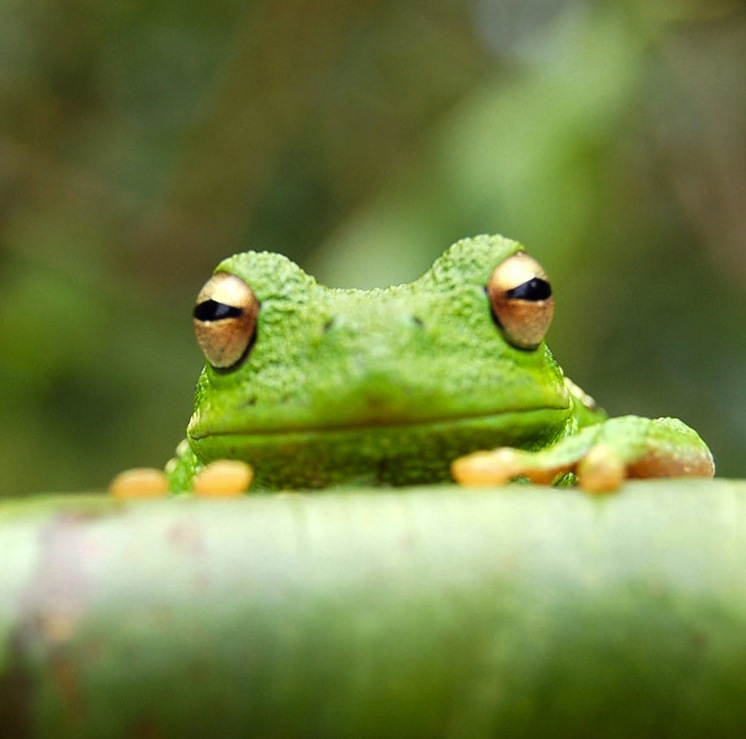
\includegraphics[width=0.5\textwidth]{frog.jpg}
\caption{\label{fig:frog}This is a figure caption.}
\end{figure}

\begin{table}
\centering
\begin{tabular}{l|r}
Item & Quantity \\\hline
Widgets & 42 \\
Gadgets & 13
\end{tabular}
\caption{\label{tab:widgets}An example table.}
\end{table}

\subsection{Mathematics}

\LaTeX{} is great at typesetting mathematics. Let $X_1, X_2, \ldots, X_n$ be a sequence of independent and identically distributed random variables with $\text{E}[X_i] = \mu$ and $\text{Var}[X_i] = \sigma^2 < \infty$, and let
$$S_n = \frac{X_1 + X_2 + \cdots + X_n}{n}
      = \frac{1}{n}\sum_{i}^{n} X_i$$
denote their mean. Then as $n$ approaches infinity, the random variables $\sqrt{n}(S_n - \mu)$ converge in distribution to a normal $\mathcal{N}(0, \sigma^2)$.

\subsection{Lists}

You can make lists with automatic numbering \dots

\begin{enumerate}
\item Like this,
\item and like this.
\end{enumerate}
\dots or bullet points \dots
\begin{itemize}
\item Like this,
\item and like this.
\end{itemize}

We hope you find write\LaTeX\ useful, and please let us know if you have any feedback using the help menu above.

\end{document}